%%=============================================================================
%% Prototype
%%=============================================================================

\chapter{Prototype}
\label{ch:prototype}

\section{Inleiding}

In dit hoofdstuk zal binnen het bestaande platform Innerdreams gamification worden geïmplementeerd, gebruik makend van DNN. Er werd gekozen om een puntensysteem, een badgesysteem, een scorebord en een beloningswinkel te implementeren. Deze elementen werden gekozen na een brainstormsessie en een kort onderzoek over de verschillende manieren waarop gamification kan worden geïmplementeerd.

\section{Gamification binnen Innerdreams}

Zoals hierboven werd vermeld, zal gamification worden geïmplementeerd. Gebruikers kunnen punten verzamelen door enquêtes in te vullen en te delen. Meer specifiek kunnen punten worden verzameld per ingevulde pagina van de enquête, per volledig ingevulde enquête, per gedeelde enquête en per gedeelde enquête die ingevuld werd. Ook kunnen gebruikers badges verzamelen als ze een mijlpaal hebben bereikt en zal een scorebord worden weergegeven met daarop de personen met het hoogste aantal punten. De verzamelde punten kunnen worden gebruikt om verschillende artikelen aan te schaffen in de beloningswinkel.

\section{Punten}

Om het puntensysteem uit te werken werd gekozen om deze te linken aan enquêtes. Zoals te zien in Figuur \ref{fig:puntendiagram} werd een tabel toegevoegd aan de SQL databank met volgende kolommen:

\begin{itemize}
    \item PuntenID: de primaire sleutel als unieke identificatie
    \item Pagina: het aantal punten dat wordt verdiend bij het volledig invullen van een pagina van een enquête.
    \item EnqueteCompleted: het aantal punten dat wordt verdiend bij het volledig voltooien van een enquête.
    \item Share: het aantal punten dat wordt verdiend bij het delen van een enquête.
    \item ShareCompleted: het aantal punten dat wordt verdiend bij het succesvol voltooien van een enquête door de persoon met wie de enquête is gedeeld.
    \item EnqueteID: de vreemde sleutel die de punten linkt aan een enquête.
\end{itemize}

\begin{figure}
    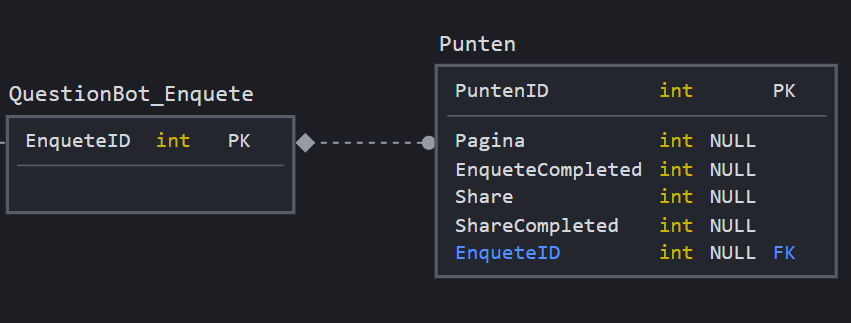
\includegraphics[width=\linewidth]{PuntenDiagram.png}
    \caption{Punten tabel.}
    \label{fig:puntendiagram}
\end{figure}

Ook was het nodig om bij de gebruikerstabel een extra kolom toe te voegen die bijhoudt hoeveel punten een gebruiker heeft, te zien in Figuur \ref{fig:gebruikerpunten}.

\begin{figure}
    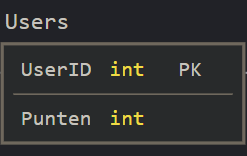
\includegraphics[width=\linewidth]{GebruikerPunten.png}
    \caption{Gebruikerspunten.}
    \label{fig:gebruikerpunten}
\end{figure}

\section{Badges}

Voor het verdienen van badges werd gekozen om deze te linken aan het totale aantal deelnames van een gebruiker aan enquêtes. In Figuur \ref{fig:badgetabel} is te zien dat een tabel werd toegevoegd aan de SQL databank met volgende kolommen:

\begin{itemize}
    \item ID: de primaire sleutel als unieke identificatie
    \item ImageLink: een verwijzing naar de afbeelding van de badge.
    \item Title: een titel die de badge beschrijft.
    \item TriggerQuery: een SQL-query die wordt uitgevoerd eenmaal aan een bepaalde voorwaarde voldaan is.
\end{itemize}

\begin{figure}
    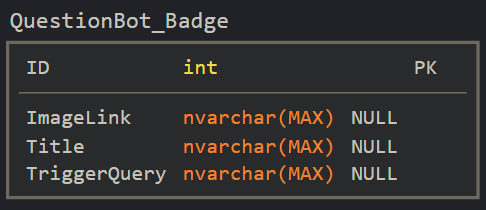
\includegraphics[width=\linewidth]{BadgeTabel.png}
    \caption{Badge tabel.}
    \label{fig:badgetabel}
\end{figure}

Eenmaal een gebruiker op de laatste pagina van een enquête terechtkomt zullen twee lijsten van badges opgehaald worden, het totale aantal badges in het systeem en de behaalde badges van de gebruiker. Deze twee lijsten zullen met elkaar vergeleken worden en als een badge wordt tegengekomen die de gebruiker nog niet heeft zal gecontroleerd worden of hij/zij aan de voorwaarden voldoet. Dit gebeurt aan de hand van een stored procedure, te zien in de volgende code \ref{lst:csb}. Binnen deze stored procedure zal de eerder vernoemde trigger query worden uitgevoerd.


\begin{lstlisting}[caption={De CheckSucceededBadge stored procedure.},
    label={lst:csb},
    language=SQL,
    showspaces=false,
    basicstyle=\ttfamily,
    numbers=left,
    numberstyle=\tiny,
    numbersep=1pt,
    breaklines=true
    commentstyle=\color{gray}]
    ALTER PROCEDURE [dbo].[QuestionBot_CheckSucceededBadge](@BadgeID int, @UserID int) as
    BEGIN
    Declare @statement as nvarchar(max) 
    set @statement = (select TriggerQuery from QuestionBot_Badge where ID = @BadgeID) 
    EXECUTE sp_executesql @statement , N'@UserID int',@UserID=@UserID
    END
\end{lstlisting}

In volgende code \ref{lst:tq} is te zien hoe zo een trigger query er uit ziet. Voor een gebruiker wordt zijn/haar totale aantal deelnames geteld aan alle enquêtes. Als dit totaal voldoet aan een bepaalde voorwaarde zal 1 worden geretourneerd, wat wil zeggen dat de gebruiker een badge heeft verdiend. Als 0 wordt geretourneerd is de voorwaarde niet voldaan. In dit voorbeeld is te zien dat voor de huidige gebruiker wordt gecontroleerd of hij/zij minstens 1 enquête heeft voltooid. Zo ja, zal deze persoon een badge verdienen met bijvoorbeeld de tekst ``Vul je eerste enquête in''.

\begin{lstlisting}[caption={De badge trigger query.},
    label={lst:tq},
    language=SQL,
    showspaces=false,
    basicstyle=\ttfamily,
    numbers=left,
    numberstyle=\tiny,
    numbersep=1pt,
    breaklines=true
    commentstyle=\color{gray}]
    declare @Participations int set @Participations = (select count(*) from QuestionBot_Participations where UserID = @UserID) 
    if (@Participations >= 1) select 1 else select 0
\end{lstlisting}

\section{Scorebord}

